%%%%%%%%%%%%%%%%%%%%%%%%%%%%%%%%%%%%%%%%%%%%%%%%%%%%%%%%%%%%%%%%%%%%%%%%%%%%%%%%%%%%%%
%%%%%%%%%%%%%%%%%%%%%%%%%%%%%%%%%%%%%%%%%%%%%%%%%%%%%%%%%%%%%%%%%%%%%%%%%%%%%%%%%%%%%%
%%%%%%%%%%%%%%%%%%%%%%%%%%%%%%%%%%%%%%%%%%%%%%%%%%%%%%%%%%%%%%%%%%%%%%%%%%%%%%%%%%%%%%
%% docART Utility - A Python/Lua(LaTeX) based tool for semi-automated documentation %%
%% Source: https://github.com/d-sacre/docart-documentation-utility/                 %%
%% Version: alpha-2022-04-30                                                        %%
%% License: GNU General Public License (GPLv3)                                      %%
%% Copyright (C) 2022 Martin Stimpfl, Daniel Sacré                                  %%
%%                                                                                  %%
%% This program is free software: you can redistribute it and/or modify             %%
%% it under the terms of the GNU General Public License as published by             %%
%% the Free Software Foundation, either version 3 of the License, or                %%
%% (at your option) any later version.                                              %%
%%                                                                                  %%
%% This program is distributed in the hope that it will be useful,                  %%
%% but WITHOUT ANY WARRANTY; without even the implied warranty of                   %%
%% MERCHANTABILITY or FITNESS FOR A PARTICULAR PURPOSE.  See the                    %%
%% GNU General Public License for more details.                                     %%
%%                                                                                  %%
%% You should have received a copy of the GNU General Public License                %%
%% along with this program.  If not, see <https://www.gnu.org/licenses/>.           %%
%%%%%%%%%%%%%%%%%%%%%%%%%%%%%%%%%%%%%%%%%%%%%%%%%%%%%%%%%%%%%%%%%%%%%%%%%%%%%%%%%%%%%%
%%%%%%%%%%%%%%%%%%%%%%%%%%%%%%%%%%%%%%%%%%%%%%%%%%%%%%%%%%%%%%%%%%%%%%%%%%%%%%%%%%%%%%
%%%%%%%%%%%%%%%%%%%%%%%%%%%%%%%%%%%%%%%%%%%%%%%%%%%%%%%%%%%%%%%%%%%%%%%%%%%%%%%%%%%%%%

\chapter{Usage}
	\label{chap:docart-usage}
	\section{Terminal/Command Line}
		\label{sec:docart-usage:command-line}
		To use the \productName~Utility in the terminal/command line, proceed as follows:
		\begin{enumerate}[label={\color{docartTurquoise}Step \arabic*:},leftmargin=*]
			\item Open a terminal/command line and set via \lstinline{cd} the working directory to the folder where your \productName~project files are located.
			\item Run the command\\[0.25cm]
			\lstinline{lualatex --shell-escape LATEXFILENAME.tex}\\[0.25cm]
			where you replace \lstinline{LATEXFILENAME} with the name of the \LaTeX-file located in the root directory of your project folder.
		\end{enumerate}
	
		\begin{daWarningBox}
			The Lua\LaTeX~command has to be run from a shell with a working directory identical to the root folder of your \productName~project.
			Even providing an absolute path like\\[0.125cm]
			\lstinline$lualatex --shell-escape /ABS/PATH/TO/LATEXFILE.tex$\\[0.125cm]
			leads to the problem that the \productName~class-file cannot be loaded.
		\end{daWarningBox}
	
		\begin{daInfoBox}
			\begin{itemize}[leftmargin=*]
				\setlength\itemsep{-0.1em}
				\item Certain elements (\mbox{e.\,g.} table of contents, references, tables etc.) need at least two compilations to be displayed properly. 
				Therefore the authors recommend to always compile twice by running \lstinline{lualatex --shell-escape LATEXFILENAME.tex} twice in succession.
				\item Running two compilations via\\[0.125cm]
				\lstinline$lualatex --shell-escape LATEXFILENAME.tex \&\&$\\  
				\lstinline$lualatex --shell-escape LATEXFILENAME.tex$\\[0.125cm]
				is not recommended. If an compilation error should occur, the compilation would restart and throwing the same error another time. This is especially not favorable if the compilation duration is long.
				\item More complex compilation pipelines for example like required for creating a bibliography can be achieved with a \mbox{\lstinline{make}-file}.
			\end{itemize}
		\end{daInfoBox}
		
	\newpage
	\section{TeXstudio}
		To use the \productName~Utility with TeXstudio, proceed as follows:
		\begin{enumerate}[label={\color{docartTurquoise}Step \arabic*:},leftmargin=*]
			\item Open the \LaTeX-file located in the root directory of your \productName~project folder with TeXstudio.
			\item To compile the \LaTeX~source code and view the pdf output in the internal pdf viewer,
			press either \lstinline{F5} on your keyboard or the \enquote{Build \& View}-button in the GUI (see \mbox{figure \ref{fig:usage:texstudio:compilation-screenshot}}).
		\end{enumerate}
		\begin{figure}[h!]
			\centering
			\begin{tikzpicture}
				\node[anchor=south west,inner sep=0] (image) at (0,0) {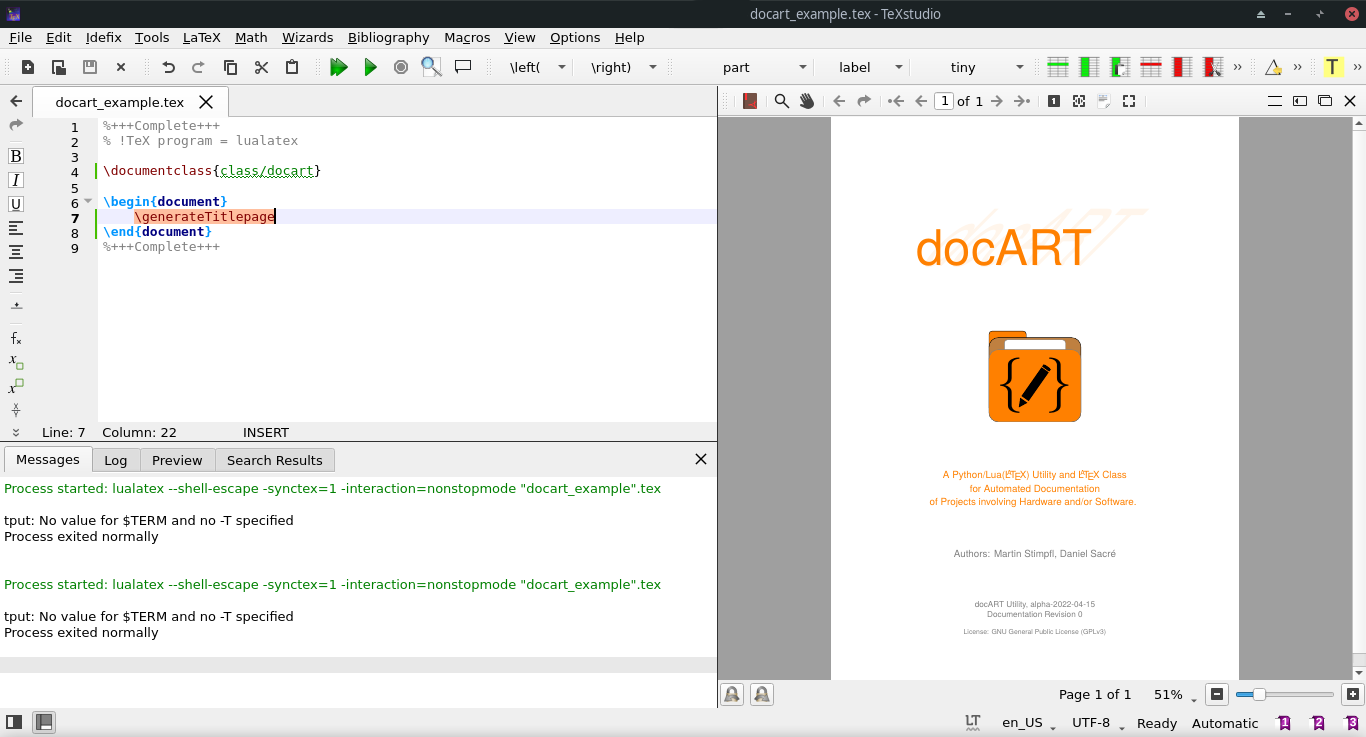
\includegraphics[width=\linewidth]{./pictures/texstudio-usage-screenshot/texstudio-usage_compilation_edited.png}};
				\begin{scope}[x={(image.south east)},y={(image.north west)}]
					\draw[orange,ultra thick](0.235,0.8875)rectangle(0.26,0.93);
					\path(0.235,0.8875)--(0.26,0.8875)node[midway,below]{\textcolor{orange}{Build \& View}};
				\end{scope}
			\end{tikzpicture}
			\caption{%
				Screenshot of the compilation of a file in TeXstudio. \LaTeX~source code (top left), \mbox{Messages}/Log/Preview/Search Results (bottom left)
				and a view of the compiled pdf (right). The \mbox{\enquote{Build \& View}-button} (top) is highlighted in orange.%
			}
			\label{fig:usage:texstudio:compilation-screenshot}
		\end{figure}
	
		\begin{daInfoBox}
			TeXstudio automatically determines the minimum necessary amount of compilations to produce a correct pdf output (including a correctly updated table of contents, tables, references, etc.). In contrary to the terminal/command line usage described in \mbox{section \ref{sec:docart-usage:command-line}}, the users do not have to determine this number by themselves. A disadvantage of using TeXstudio over the terminal/command line is that the compilation takes longer and the error messages might not be as precise/immediate.
		\end{daInfoBox}
	
%	